%%%%%%%%%%%%%%%%%%%%%%%%%%%%%%%%%%%%%%%%%
% Beamer Presentation
% LaTeX Template
% Version 1.0 (10/11/12)
%
% This template has been downloaded from:
% http://www.LaTeXTemplates.com
%
% License:
% CC BY-NC-SA 3.0 (http://creativecommons.org/licenses/by-nc-sa/3.0/)
%
%%%%%%%%%%%%%%%%%%%%%%%%%%%%%%%%%%%%%%%%%

%----------------------------------------------------------------------------------------
%	PACKAGES AND THEMES
%----------------------------------------------------------------------------------------

\documentclass{beamer}

\mode<presentation> {

% The Beamer class comes with a number of default slide themes
% which change the colors and layouts of slides. Below this is a list
% of all the themes, uncomment each in turn to see what they look like.

%\usetheme{default}
%\usetheme{AnnArbor}
%\usetheme{Antibes}
%\usetheme{Bergen}
%\usetheme{Berkeley}
%\usetheme{Berlin}
%\usetheme{Boadilla}
%\usetheme{CambridgeUS}
%\usetheme{Copenhagen}
%\usetheme{Darmstadt}
%\usetheme{Dresden}
%\usetheme{Frankfurt}
%\usetheme{Goettingen}
%\usetheme{Hannover}
%\usetheme{Ilmenau}
%\usetheme{JuanLesPins}
%\usetheme{Luebeck}
\usetheme{Madrid}



%\usetheme{Malmoe}
%\usetheme{Marburg}
%\usetheme{Montpellier}
%\usetheme{PaloAlto}
%\usetheme{Pittsburgh}
%\usetheme{Rochester}
%\usetheme{Singapore}
%\usetheme{Szeged}
%\usetheme{Warsaw}

% As well as themes, the Beamer class has a number of color themes
% for any slide theme. Uncomment each of these in turn to see how it
% changes the colors of your current slide theme.

%\usecolortheme{albatross}
%\usecolortheme{whale}
%\usecolortheme{beetle}
%\usecolortheme{crane}
%\usecolortheme{dolphin}
%\usecolortheme{dove}
%\usecolortheme{fly}
%\usecolortheme{lily}
%\usecolortheme{orchid}
%+\usecolortheme{rose}
%\usecolortheme{seagull}
%\usecolortheme{seahorse}
%\usecolortheme{whale}
%\usecolortheme{wolverine}
\usecolortheme{beaver}

%\setbeamertemplate{footline} % To remove the footer line in all slides uncomment this line
\setbeamertemplate{footline}{\hspace{0.97\paperwidth}\vspace*{0.1cm}\scriptsize\insertpagenumber} % To replace the footer line in all slides with a simple slide count uncomment this line
\setbeamertemplate{navigation symbols}{} % To remove the navigation symbols from the bottom of all 

\setbeamertemplate{section in toc}[ball unnumbered]

}
%\usefonttheme[onlymath]{serif}			% para fontes matemáticas

\usepackage{booktabs} % Allows the use of \toprule, \midrule and \bottomrule in tables
%\usepackage[brazil]{babel}		% Idioma do documento
\usepackage[T1]{fontenc}		% Selecao de codigos de fonte.
\usepackage{graphicx}			% Inclusão de gráficos
\usepackage[utf8]{inputenc}		% Codificacao do documento (conversão automática dos acentos)
\usepackage[citestyle=authoryear,bibstyle=authoryear,backend=bibtex]{biblatex}
\usepackage{pdfpages}
\usepackage{lmodern}
\usepackage[lined, linesnumbered]{algorithm2e}
\usepackage{media9}
\usepackage{adjustbox} % for adjincludegraphics
\setbeamertemplate{caption}[numbered]
\usepackage{tikz}
\usepackage{subfig}
\graphicspath{{images/}}
\renewcommand{\footnotesize}{\scriptsize}
\usetikzlibrary{mindmap}
\usepackage{multirow}
\renewcommand*{\nameyeardelim}{\addcomma\addspace}


\addbibresource{library.bib}
%----------------------------------------------------------------------------------------
%	TITLE PAGE
%----------------------------------------------------------------------------------------

\title{A Deep Learning Approach to Generate Offline Handwritten Signatures Based on Online Samples} % The short title appears at the bottom of every slide, the full title is only on the title page
\vspace{0.4in}
\author[]{ Victor Kléber Santos Leite Melo \\ {\footnotesize\texttt{vkslm@ecomp.poli.br}} \\
\vspace{0.2in}
Advisor: Prof. Dr. Byron Leite Dantas Bezerra \\
Co-Advisor: Prof. Dr. Giuseppe Pirlo}


\date{\today} % Date, can be changed to a custom date

\begin{document}

\begin{frame}

\begin{minipage}{1\linewidth}
  \centering


  \begin{tabular}{cc}
	\begin{tabular}{c}
		\includegraphics[width=1.0cm]{imagens/brasao.pdf}
		\hspace{0.2cm}
		\includegraphics[width=2.0cm]{imagens/ecomp.pdf}
	\end{tabular}

    \begin{tabular}{c}
      \textbf{Universidade de Pernambuco - UPE} \\ \textbf{Escola Politécnica de Pernambuco - POLI} \\ \textbf{Mestrado em Engenharia da Computação}
    \end{tabular}
  \end{tabular}
\end{minipage}

\titlepage
\end{frame}

%----------------------------------------------------------------------------------------
%	PRESENTATION SLIDES
%----------------------------------------------------------------------------------------




%------------------------------------------------

%------------------------------------------------


\begin{frame}
\frametitle{Introduction}

\centering
Biometric technology is used in several security applications for personal authentication. 
\begin{figure}[!htb]
\centering


\pause
 \subfloat[Fingerprint]{\includegraphics[height=0.2\textheight, width=0.16\textwidth]{slides/fingerprint}} 
\hspace*{0.1in} % separation between the subfigures
 \subfloat[Iris]{\includegraphics[height=0.2\textheight, width=0.15\textwidth]{slides/iris}} 
\hspace*{0.1in}% separation between the subfigures
\subfloat[Handwritten Signature]{\includegraphics[height=0.2\textheight, width=0.30\textwidth]{signature2}} 
\hspace*{0.1in}% separation between the subfigures
 \subfloat[Voice]{\includegraphics[height=0.2\textheight, width=0.27\textwidth]{slides/voice}} 
 
\caption{Some biometric traits used for person authentication. } %\label{fig:activation}



\end{figure}
\pause
\begin{block}{Biometry Categories}
\begin{itemize}
\item Physiological - biological characteristics such as fingerprint, palm print, iris, face.
\item Behavioral - individual acquired traits such as voice pattern and handwritten signature. 

\end{itemize}

\end{block}



\end{frame}


\begin{frame}
\frametitle{Handwritten Signature}
\begin{figure}[!htb]
\centering
 \subfloat{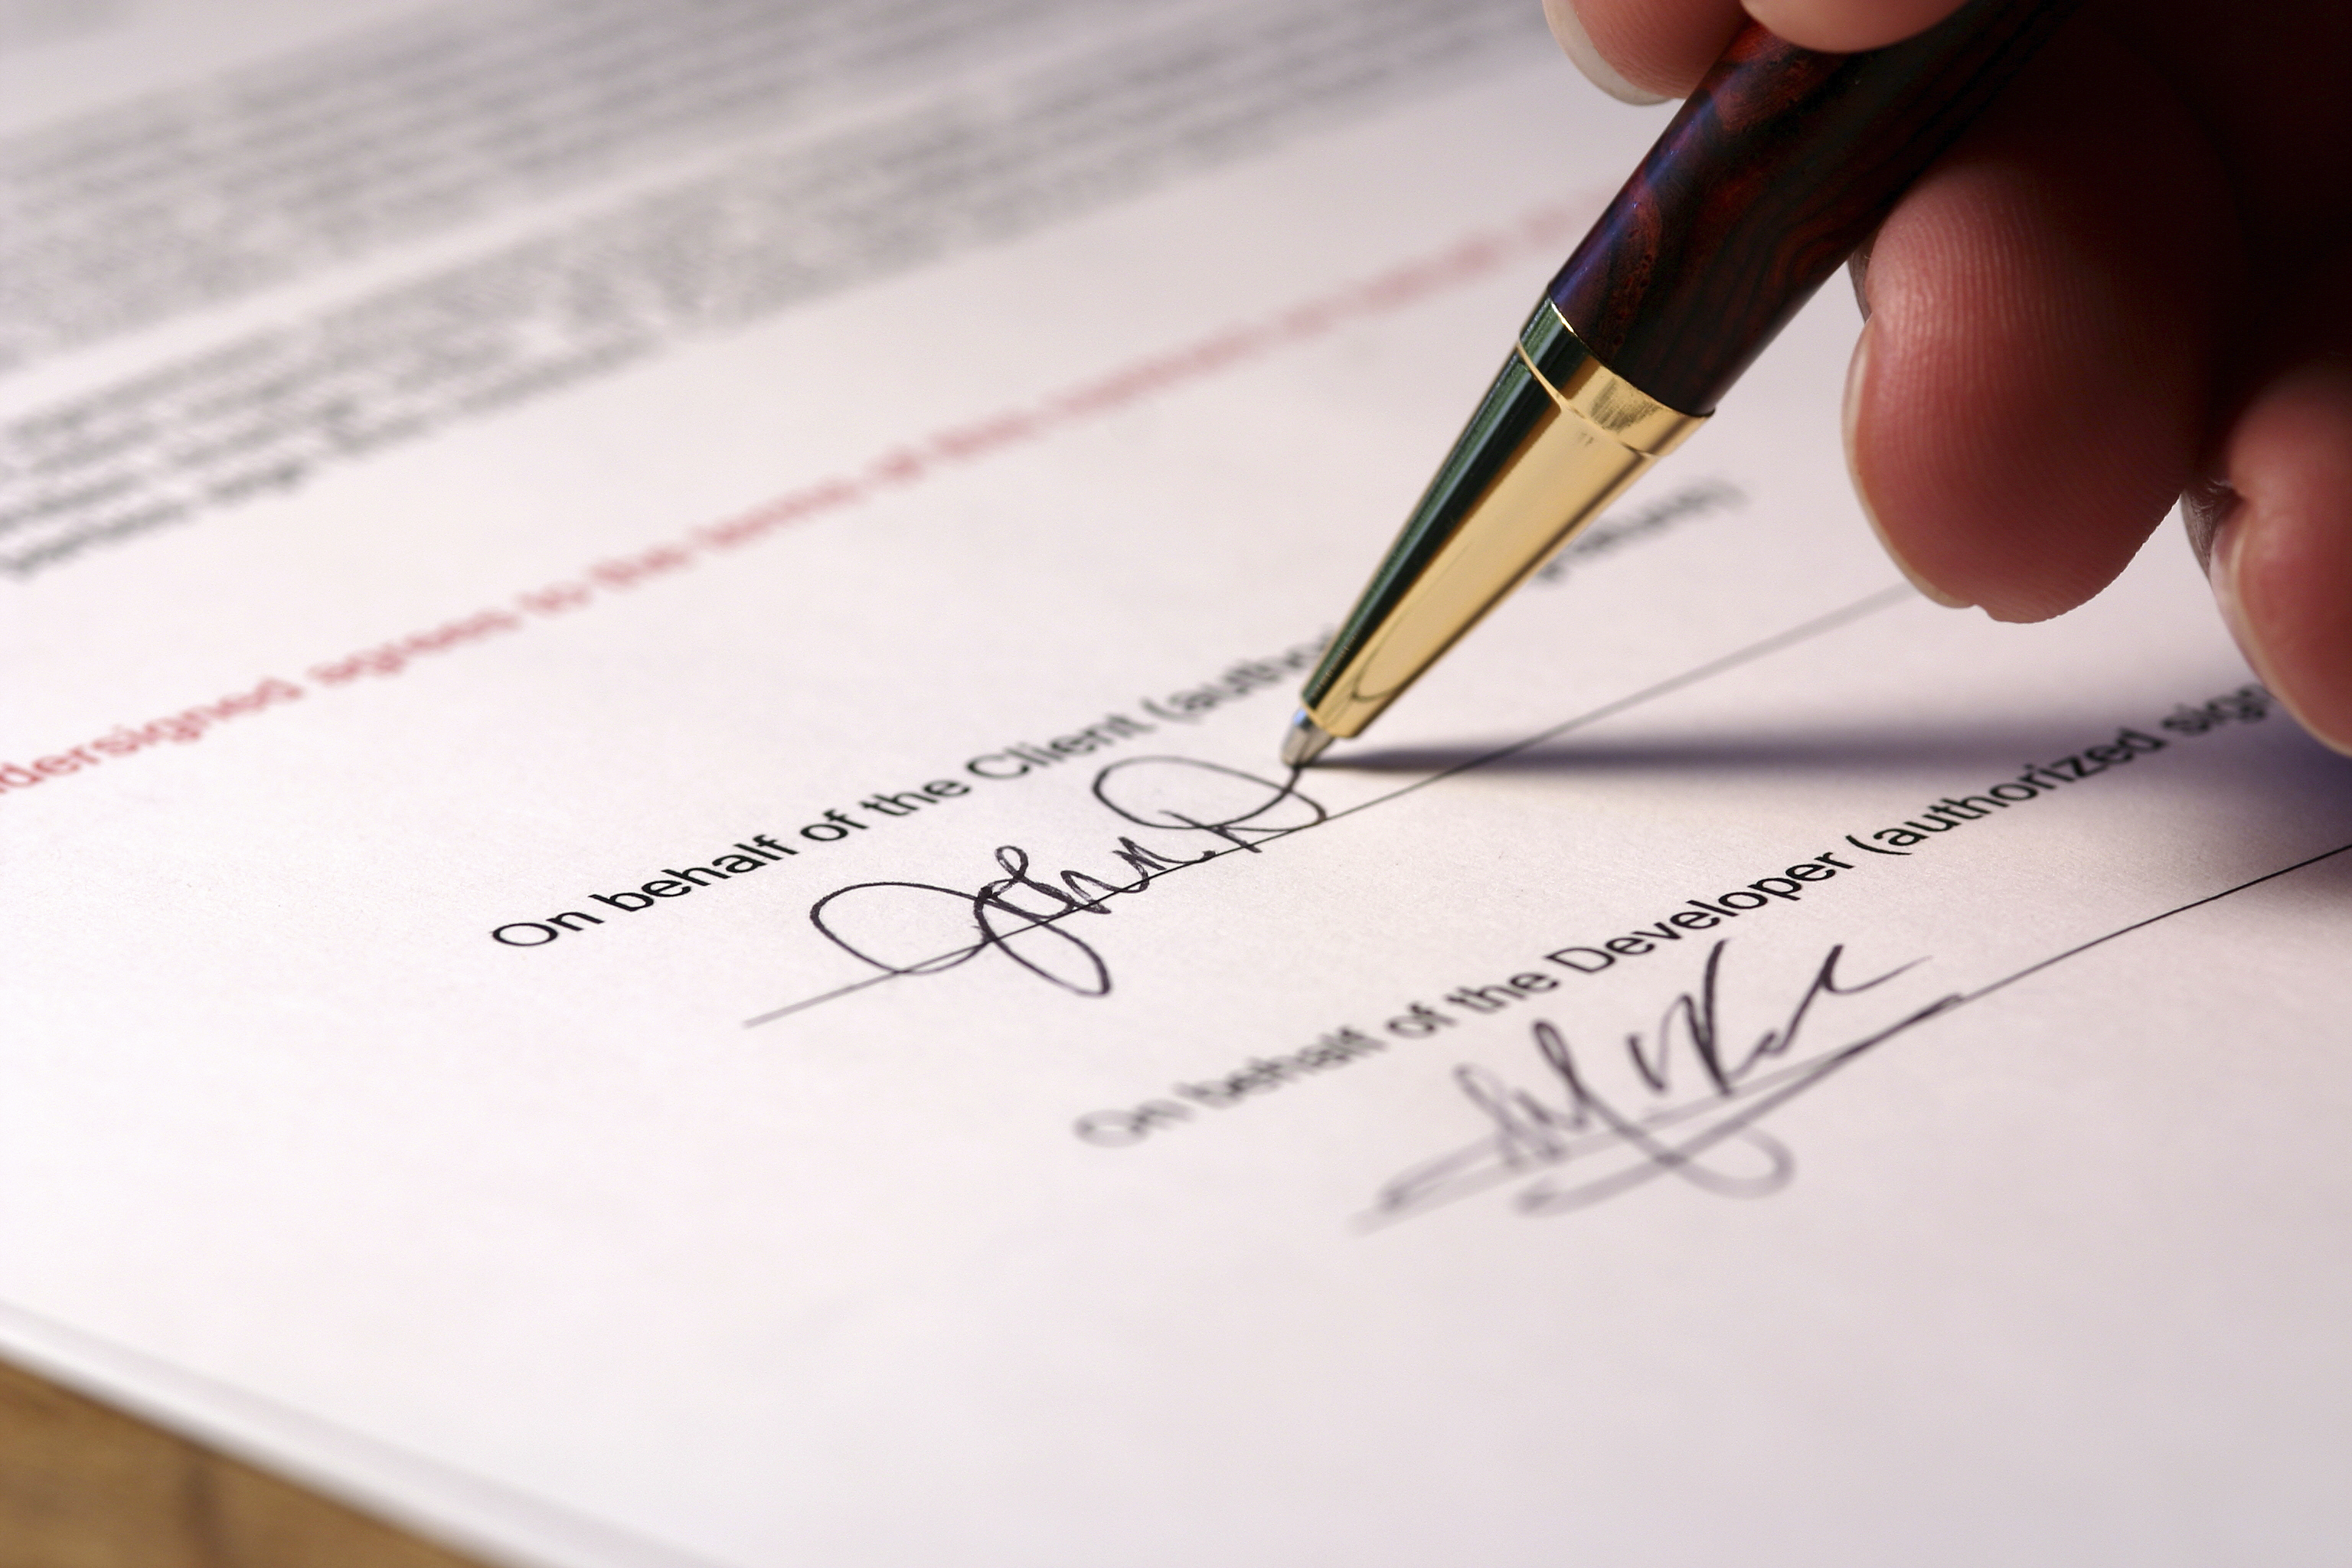
\includegraphics[width=0.32\textwidth]{slides/signing1}} 
\hspace*{0.1in} % separation between the subfigures
 \subfloat{\includegraphics[width=0.32\textwidth]{slides/sigbiometry}} 
\hspace*{0.1in}% separation between the subfigures
\subfloat{\includegraphics[ width=0.3\textwidth]{slides/signing2}} 

 
\caption{Handwritten Signatures are widespread biometry.}  %\label{fig:activation}

\end{figure}
\end{frame}


\begin{frame}
\frametitle{Handwritten Signature (2)}

\textbf{The Handwritten Signature widespread can be attributed to \footfullcite{impedovo2008state}:}
\begin{itemize}
\item Signature acquisition is easy and non-invasive;
\item Most individuals are familiar with its use in their daily life;
\item Signatures can be employed as a sign of confirmation in a wide variety of documents, namely, bank checks, identification documents and a variety of business certificates and contracts.
\end{itemize}
\end{frame}

\begin{frame}
\frametitle{Overview of a Handwritten Signature Verification System}
\begin{figure}[!htb]
\centering
\includegraphics[width=\textwidth]{biometry-overview}
\caption{Overview of a typical handwritten signature based system. Figure adapted from \parencite{jain2016} \footfullcite{jain2016}.}
\label{fig_ahsv-overview}
\end{figure}

\end{frame}

\begin{frame}
\frametitle{Overview of a Handwritten Signature Verification System}
\begin{figure}[!htb]
\centering
\includegraphics[width=\textwidth]{biometryoverview2}

\label{fig_ahsv-overview}
\end{figure}

\end{frame}


\begin{frame}
\frametitle{Overview of a Handwritten Signature Verification System}
\begin{figure}[!htb]
\centering
\includegraphics[width=\textwidth]{biometryoverview3}

\label{fig_ahsv-overview}
\end{figure}

\end{frame}



\begin{frame}
\frametitle{Overview of a Handwritten Signature Verification System}
\begin{figure}[!htb]
\centering
\includegraphics[width=\textwidth]{biometryoverview4}

\label{fig_ahsv-overview}
\end{figure}

\end{frame}


\begin{frame}
\frametitle{Overview of a Handwritten Signature Verification System}
\begin{figure}[!htb]
\centering
\includegraphics[width=\textwidth]{biometryoverview5}

\label{fig_ahsv-overview}
\end{figure}

\end{frame}

\begin{frame}
\frametitle{Online vs Offline Handwritten Signatures}

\begin{figure}[!htpb]
\begin{block}{OFFLINE -> STATIC}
An optical scanner is used to obtain the signature directly from the pen on the paper, and only the digital image of the signature is available.
\end{block}

\begin{block}{ONLINE -> DYNAMIC}
Data is stored during the writing process and consists of a temporal sequence of the two-dimensional coordinates $(x, y)$ of consecutive points. 
\end{block}
\centering
 \subfloat[A signature scanned from paper]{\includegraphics[width=0.3\textwidth]{signature.PNG}} 
\hspace*{0.5in} % separation between the subfigures
\subfloat[Digitizing tablet Wacom STU-500] {\includegraphics[width=0.3\textwidth]{stu500.jpg}}
\caption{Different signature acquisition methods. } \label{fig:acquisition}
\end{figure}
\end{frame}

\begin{frame}
\frametitle{Online vs Offline Handwritten Signatures (2)}

\begin{figure}[!htpb]

\centering
 \subfloat{\includegraphics[height=0.45\textwidth]{slides/online}} 
\hspace*{0.1in} % separation between the subfigures
\subfloat {\includegraphics[height=0.4\textwidth]{slides/offline}}
\caption{An online and the respective offline signature sample. Extracted from \parencite{galbally2015line} }
\end{figure}
\end{frame}


\begin{frame}
\frametitle{Online vs Offline Handwritten Signatures (3)}


\begin{block}{ONLINE MODALITY}
Does not convey information about:
\begin{itemize}
\item The overall shape of the signature;
\item The width of the strokes;
\item The texture of the ink on the paper.
\end{itemize}
\end{block}

\pause

\begin{block}{OFFLINE MODALITY}
\begin{itemize}
\item Lost all dynamic information about the signature;
\item Dynamic features can only be inferred from a static image \parencite{nel2005estimating}. 
\end{itemize}



\end{block}

\end{frame}

\begin{frame}
\frametitle{Handwritten Signature Intra-personal variability}
\begin{figure}[!h]
\centering
\includegraphics[width=0.8\textwidth]{superimposed}
\caption{Superimposed genuine signatures of the same writer. A high intra-personal variability can be noticed. Extracted from \parencite{hafemann2015offline}. }
\label{fig:intraclass}
\end{figure}

\end{frame}

\begin{frame}
\frametitle{Handwritten Signature Inter-personal variability}
\begin{figure}[!htb]
\centering
\includegraphics[width=\textwidth]{forgeries}
\end{figure}

The first column of signatures are genuine references, the following three samples are questioned signatures \footnote{From left to right, top to bottom (F means Forgery and G means Genuine): FGF FFG GFF}. Signature images extracted from \parencite{mcyt-100}.
\end{frame}


\begin{frame}
\frametitle{Types of Forgeries}
In the field of signature verification, forgeries are usually classified into two types \parencite {impedovo2008state}. 
\begin{itemize}
\item The first one is the random forgery which is created in a situation which an impostor who has no information about the person or the shape of the original signature tries to verify the identity of a signer using his signature instead of the signature to be tested. The forger does not attempt to simulate or trace a genuine signature.

\item The second type is the skilled forgery, in which the forger tries and practices imitating as closely as possible the static and dynamic information of the genuine signature model. The forger has access for both the user’s name and signature and tries to reproduce it with a similar intra-class variability.
\end{itemize}
\end{frame}


\begin{frame}
\frametitle{Data in Signature Verification}

The performance of signature verification systems can be improved by increasing the number of samples in the training dataset. The amount of data available for each user is often insufficient in real applications. During the enrollment phase,
users are often required to supply only a few samples of their signatures. In other words, even if there is a significant number of users enrolled in the system, a classifier needs to perform well for a new user, for whom only a small set of samples are available. Since the acquisition and distribution of real signatures arise legal and privacy concerns \parencite{diaz2014generation}, the use of realistic synthetic signatures could be
regarded as a good alternative. 

\end{frame}


\begin{frame}
\frametitle{Synthetic Samples}

The use of realistic synthetic signatures could be regarded as a good alternative. As a consequence, over the last years, several works on both online \parencite{galbally2009synthetic, galbally2012synthetic} and offline \parencite{ferrer2013synthetic, ferrer2013realistic} signature synthesis have been carried out. These synthetically generated signatures show a similar behavior to real ones, thus enabling to enlarge existing databases and offering new possibilities for offline recognition.

\end{frame}

\begin{frame}
\frametitle{Online to Offline}
Some efforts have been performed on the generation of synthetic static data taking into account dynamic features during the synthesis process \parencite{diaz2014generation}. Among others, this type of synthesis approach presents some practical applications:
\begin{itemize}
  \item generation of synthetic static samples to be fused with the original online signatures in order to improve the performance in an online verification scenario;
  \item enlargement of existing offline signature databases;
  \item development of systems capable of integrating both online and offline samples interchangeably, towards a unified signature biometry \parencite{chapter}.
\end{itemize}
\end{frame}

\begin{frame}
\frametitle{Goal}


In contrast to the models proposed in the literature \parencite{ferrer2013synthetic, ferrer2013realistic, diaz2014generation}, the approach presented in this work is designed under the perspective of supervised training. 

\textit{"The goal of this work is to design an approach to generate synthetic offline handwriting signatures based on online data, modeling this problem as a supervised machine learning task, through a Deep Convolutional Neural Network, in order to enlarge offline signature datasets to improve offline signature verification systems recognition rates."}

This statement is developed through the following actions:
\begin{itemize}
\item Creation and training of a Deep Neural Network model able to translate dynamic handwritten information into an offline manuscript
\item Generation of an offline synthetic dataset based on a publicly available online signature dataset
\item Comparison of the proposed approach’s performance with a state-of-the-art method to evaluate the closeness of synthetic signatures with respect to real signatures. 
\end{itemize}
\end{frame}




\begin{frame}
\frametitle{Contents} % Table of contents slide, comment this block out to remove it
\tableofcontents % Throughout your presentation, if you choose to use \section{} and \subsection{} commands, these will automatically be printed on this slide as an overview of your presentation
\end{frame}
%----------------------------------------------------------------------------------------

\section{Off-line Signature Synthesis Using On-line Samples}
\begin{frame}
\frametitle{Off-line Signature Synthesis Using On-line Samples}
According to \parencite{guest2013assessment}, although online samples can be stored as a time-series for use in any form of an AHSVS, there are situations where it might be needed to represent the data as an image reproducing the original static signature. 
\end{frame}

\section{Neural Networks and Deep Learning}

\begin{frame}
\frametitle{Neural Networks}
The human brain is a complex, non-linear and parallel ``computer'' consisting of \textbf{millions of connected neurons} \parencite{haykin2009neural}.
\end{frame}

\begin{frame}
\frametitle{Perceptron}
\begin{figure}[!htb]
\centering
\includegraphics[width=0.8\textwidth]{perceptron}
\caption{Perceptron representation. $x_{1}$ and $x_{2}$ represent the input signal, $b$ the bias term, $w_{0}$, $w_{1}$, $w_{2}$ the weights, $f_{\:\sum}$ is the activation function (in this case, a step function) and the output signal is given by $y$.}
\label{perceptron}
\end{figure}
\end{frame}

\begin{frame}
\frametitle{Multilayer Perceptron}
\begin{figure}[!htb]
\centering
\includegraphics[height=0.7\textheight]{mlp}
\caption{Each layer contains several perceptron units, which are then connected to units in the subsequent layer.}
\label{mlp}
\end{figure}
\end{frame}

\begin{frame}
\frametitle{Multilayer Perceptron}
An MLP can be thought of as a function that maps from input to output vectors, parameterized by the neuron connection weights. The output of a layer
is calculated by applying the neuron activation function for all neurons on the layer, as
noted below
\begin{equation}
y^{(l)} = f(W^{(l)} y^{(l-1)} + b^{(l)})
\label{eq:outputmlp}
\end{equation}
where $W^{(l)}$ is a matrix of weights assigned to each pair of neurons from layer $l$ and $l-1$, and $b^{(l)}$ is a vector of bias terms for each neuron in layer $l$. Calculating the output starting from the first hidden layer, up to the output layer is also referred to as the \textit{forward propagation} phase.
\end{frame}

\section{Proposed Method}
\begin{frame}
\frametitle{Outline of the Proposed Method}
\begin{figure}[!htb]
\centering
\includegraphics[width=0.8\textwidth]{method}
% where an .eps filename suffix will be assumed under latex, 
% and a .pdf suffix will be assumed for pdflatex; or what has been declared
% via \DeclareGraphicsExtensions.
\caption{The proposed approach diagram and an example of the synthetic signature generation.}
\label{fig_approach}
\end{figure}
\end{frame}

\begin{frame}{Training Data}


\begin{figure}[!htb]
\centering
\includegraphics[height=0.82\textheight]{dualonoff}

\caption{Figure extracted from \parencite{galbally2015line}}
\label{fig:dualonoff}
\end{figure}
\end{frame}

\begin{frame}{Training Data}
Dual modal signature datasets (BiosecurID, Biomet, MyIdea, Sigcomp2009, Sigma, SigwiComp2013, SigWiComp2015)  had not this characteristic satisfied. Both of the representations of the signatures do not match if we plot it in a single image.

\begin{figure}[!htb]
\centering
\includegraphics[width=0.5\textwidth]{onoff}
% where an .eps filename suffix will be assumed under latex, 
% and a .pdf suffix will be assumed for pdflatex; or what has been declared
% via \DeclareGraphicsExtensions.
\caption{A sample from the BiosecurID dataset. Here we can see that the online signature (interpolated in red) can not be projected in the respective offline version.}
\label{fig:onoff}
\end{figure}
\end{frame}

\begin{frame}{Training Data}
The dual domain IRONOFF \parencite{viard1999ireste} handwriting dataset was thus used to train our model. Besides acquiring both domains of the handwriting manuscript, the online data is mapped to the same coordinate system of the offline data.

Using this dataset, we make the fair assumption that a handwritten signature is a manuscript. With that in mind, we expect that even if the network was trained on handwriting manuscripts, it would work for online signatures to generate its static version.

The IRONOFF dataset contains a total of 23000 mapped online and offline samples of the manuscripts. The offline handwriting signals have been sampled with a spatial resolution of 300 dots per inch (DPI), with 8 bits per pixel (256 gray level).

\begin{figure}[!htb]
\centering
\includegraphics{ironoff-mapped}
% where an .eps filename suffix will be assumed under latex, 
% and a .pdf suffix will be assumed for pdflatex; or what has been declared
% via \DeclareGraphicsExtensions.
\caption{An offline manuscript mapped with the respective online trajectory. Image extracted from \cite{viard1999ireste}.}
\label{fig:ironoff-mapped}
\end{figure}
\end{frame}


\begin{frame}{Preprocessing}
\begin{figure}[!htpb]
\centering
 \subfloat[input]{\includegraphics[width=2.0in]{input-ironoff}} 
\hspace*{0.5in} % separation between the subfigures
\subfloat[ground truth] {\includegraphics[width=2.0in]{gt-ironoff}}
\caption{Preprocessed data used during the training phase. (a) is the interpolated online sample, used as input and (b) is the expected prediction from the neural network, the ground truth. } \label{fig_ironoff}
\end{figure}
\end{frame}



\begin{frame}
\frametitle{Training results}
\begin{figure}[!htpb]
\centering
\subfloat{\includegraphics[scale=0.3]{samples/0}} 
\hspace*{0.4in} % separation between the subfigures
\subfloat{\includegraphics[scale=0.3]{samples/00}}
\\
\subfloat{\includegraphics[scale=0.3]{samples/4}} 
\hspace*{0.4in} % separation between the subfigures
\subfloat{\includegraphics[scale=0.3]{samples/04}}
\\
\subfloat{\includegraphics[scale=0.3]{samples/10}} 
\hspace*{0.4in} % separation between the subfigures
\subfloat{\includegraphics[scale=0.3]{samples/010}}
\\
\subfloat{\includegraphics[scale=0.3]{samples/23}} 
\hspace*{0.4in} % separation between the subfigures
\subfloat{\includegraphics[scale=0.3]{samples/023}}
\\
\addtocounter{subfigure}{-8}
\subfloat{\includegraphics[scale=0.3]{samples/30}}
\hspace*{0.4in} % separation between the subfigures
\subfloat{\includegraphics[scale=0.3]{samples/030}} 


\caption{A not cherry-picked selection of synthetic manuscripts produced using our proposed method (left) alongside the expected output (right).} \label{fig:resultingsamples}
\end{figure}
\end{frame}



\section{Evaluation Setup}

\begin{frame}
\frametitle{Evaluation Setup}
In order to evaluate the quality of the synthetic signatures generated by our system we follow the same protocol presented on the work of Diaz \textit{et al.} \cite{diaz2014generation}. Namely, we use a state-of-the-art offline verification system and a dataset comprising both online and offline signatures in order to train the verification system to evaluate the synthetic signatures.

The goal of the experiments is to measure the quality of the synthetic signatures taking into account an offline verification system performance. The questions raised are 

\begin{itemize}
  \item is the synthetic signatures system performance similar to the offered by real offline signatures?
  \item is it feasible to increase the number of samples at the enrollment stage with our proposed method synthetic signatures? 
\end{itemize}
\end{frame}

\begin{frame}{Offline signature verification system}
\section{Off-line signature verification system}
The system used for the evaluation of the real and synthetic signatures is a Linear SVM classifier and with a state-of-the-art feature extraction approach  \cite{hafemann2017learning}. The feature extraction system \footnote{https://www.etsmtl.ca/Unites-de-recherche/LIVIA/Recherche-et-innovation/Projets/Signature-Verification} uses ideas from transfer learning and multi-task learning to learn features using Convolutional Neural Networks (CNN). As discussed in Chapter before, one of the advantages of using deep learning techniques is that some models, such as the CNN, can learn filters that can be used as feature extractors. The offline system's feature extractor takes advantage of this concept.
\end{frame}

\begin{frame}{Database}
The evaluation experiments were carried out on the BiosecurID database \cite{biosecurid}. This multimodal database was made publicly available containing signatures of 132 subjects. Signatures were captured using a special digital inking pen on a paper placed over a digitizing tablet, exactly as shown in Figure \ref{fig:onoff}. Consequently, both versions, online and offline, of the same real signature were acquired at the same time. This characteristic, therefore, makes BiosecurID the ideal benchmark for the experimental evaluation conducted in this work.


The signatures samples were captured in 4 different sessions, distributed over four months. Each subject signed 4 times and forged 3 signatures per session, thus leading to each subject having 4 genuine signatures x 4 sessions = 16 genuine samples and 3 signature forgeries x 4 sessions = 12 skilled forgeries.

Since the offline signature verification system is trained with both positive and negative samples, to ensure an unbiased result towards the dataset selection, similar to the protocol followed by \cite{diaz2014generation} we used the MCYT database \cite{mcyt-100} as the negative dataset samples. The MCYT dataset includes 75 signers each with 15 genuine and 15 skilled forged signatures. The amount of negative samples was set to 25 random samples from the MCYT dataset.
\end{frame}

\begin{frame}{Experiments Protocol}
We follow the same experiment protocol proposed by \cite{diaz2014generation}. 
Two different experiments are carried out. 

\begin{itemize}
\item Experiment 1 focus on evaluating the synthetic signatures performance in comparison to real signatures
\item Experiment 2 evaluates the feasibility of synthetically increasing the number of samples available in a dataset.
\end{itemize}

For both experiments, the BiosecurID dataset is split into two subsets. The first 90 users are separated as the enrollment set, used to compute the genuine and skilled impostor scores. The remaining 42 authors are considered as the test set and are used to compute the random impostor scores. The performance is evaluated regarding the equal error rate (EER), which is the point in the Detection Error Tradeoff curve (DET) where the false acceptance rate equals the false rejection rate.
\end{frame}

\begin{frame}{Experiments Protocol}
We follow the same experiment protocol proposed by \cite{diaz2014generation}. 
Two different experiments are carried out. 

\begin{itemize}
\item Experiment 1 focus on evaluating the synthetic signatures performance in comparison to real signatures
\item Experiment 2 evaluates the feasibility of synthetically increasing the number of samples available in a dataset.
\end{itemize}
\end{frame}

\begin{frame}{Experiment 1}
\begin{figure}[!htb]
\centering
\includegraphics[width=\textwidth]{multi-and-mono}
% where an .eps filename suffix will be assumed under latex, 
% and a .pdf suffix will be assumed for pdflatex; or what has been declared
% via \DeclareGraphicsExtensions.
\caption{The proposed approach diagram and an example of the synthetic signature generation.}
\label{fig:multiandmono}
\end{figure}
\end{frame}

\begin{frame}{Experiment 2}
This experiment is designed to assess whether synthetically increasing the enrollment dataset leads to a better recognition performance. Three different enrollment sets are considered in this experiment: 
\begin{itemize}
  \item 4 real samples belonging to the
  first acquisition session
  \item 8 real samples belonging to the first and
  the second sessions
  \item 4 real samples belonging
  to the first session plus 4 synthetic samples belonging
  to the second session.
\end{itemize}
\end{frame}

\section{Results}
\begin{frame}{Results}
The goal of the experiments are:
\begin{itemize}
  \item Measure the quality of the synthetic images;
  \item Assess whether using synthetic signatures effects the recognition performance of an offline signature verification system; and
  \item Analyze the feasibility of using real and synthetic signatures
  on the enrollment set.
\end{itemize}

We compare our results with a state-of-the-art method, particularly the approach proposed by Diaz \textit{et al.} \cite{diaz2014generation}. Specifically, our proposed method is compared with the ``Image enhanced'' synthetic signatures made available as part of the BiosecurID \cite{biosecurid} dataset. The reported EER is achieved for both approaches in the same experimental conditions.

The recognition rates of three types of offline signatures are reported: 
\begin{itemize}
  \item real offline signatures, which are the corresponding real offline samples of the online signatures used to generate the synthetic samples, they serve us as a ground-truth, i.e., the ideal synthetic signature should be similar to it;
  \item synthetic signatures generated with the method proposed by Diaz \textit{et al.} \cite{diaz2014generation};
  \item synthetic signatures created with our proposed method
\end{itemize}.
\end{frame}

\begin{frame}{Experiment 1}
\begin{table}[!htb]
%% increase table row spacing, adjust to taste
\renewcommand{\arraystretch}{1.3}
% if using array.sty, it might be a good idea to tweak the value of
% \extrarowheight as needed to properly center the text within the cells
\caption{EER for real, synthetic samples from Diaz \textit{et al.} \cite{diaz2014generation} and our proposed method synthetic offline signatures, for all the approaches considered under the two possible scenarios (i.e., random and skilled forgeries)}
\label{exp1_results_table}
\centering
%% Some packages, such as MDW tools, offer better commands for making tables
%% than the plain LaTeX2e tabular which is used here.
\begin{tabular}{|l|l|l|l|}
    \hline
    \multicolumn{1}{|c|}{\multirow{2}{*}{\textbf{Mode}}} & \multicolumn{3}{c|}{\textbf{Skilled Forgeries}}          \\ \cline{2-4} 
    \multicolumn{1}{|c|}{}                               & \textbf{Real} & \textbf{Diaz \textit{et al.}} & \textbf{Proposed method} \\ \hline
    \textbf{mono-session}                                & 20.28\%            & 23.19\%            & 18.38\%                       \\ \hline
    \textbf{multi-session}                               & 17.59\%            & 22.27\%            & 16.48\%                       \\ \hline
    \multirow{2}{*}{}                                    & \multicolumn{3}{c|}{\textbf{Random Forgeries}}           \\ \cline{2-4} 
    & \textbf{Real} & \textbf{Diaz \textit{et al.}} & \textbf{Proposed method} \\ \hline
    \textbf{mono-session}                                & 9.07\%            & 10.65\%            & 9.99\%                       \\ \hline
    \textbf{multi-session}                               & 5.60\%            & 10.00\%            & 6.48\%                       \\ \hline
\end{tabular}

\end{table}
\end{frame}



\begin{frame}{Experiment 1}
\begin{figure}[!htb]
    \centering
    \includegraphics[width=1.05\textwidth]{rocs/experiment1}
    % where an .eps filename suffix will be assumed under latex, 
    % and a .pdf suffix will be assumed for pdflatex; or what has been declared
    % via \DeclareGraphicsExtensions.
    \caption{DET curves for real offline signatures and synthetic signatures (from Diaz \textit{et al.} and our proposed method), for the first experiment (mono-session and multi-session enrollment), for the two scenarios considered (random and skilled impostors)}
    \label{exp1}
\end{figure}
\end{frame}

\begin{frame}{Experiment 1 - running 30 times}
\begin{figure}[!htb]
\centering
 \subfloat[mono-session - random forgeries]{\includegraphics[width=1in]{boxplot/mono-random.png}} 
\hspace*{0.1in} % separation between the subfigures
\subfloat[mono-session - skilled forgeries] {\includegraphics[width=1in]{boxplot/mono-skilled.png}}
\hspace*{0.2in} % separation between the subfigures
\subfloat[multi-session - random forgeries]{\includegraphics[width=1in]{boxplot/multi-random.png}} 
\hspace*{0.1in} % separation between the subfigures
\subfloat[multi-session - skilled forgeries] {\includegraphics[width=1in]{boxplot/multi-skilled.png}}
\caption{Boxplot comparison for running 30 times the Experiment 1}
\end{figure}
\end{frame}

\begin{frame}{Experiment 2}

\begin{table}[!htb]
    %% increase table row spacing, adjust to taste
    \renewcommand{\arraystretch}{1.3}
    % if using array.sty, it might be a good idea to tweak the value of
    % \extrarowheight as needed to properly center the text within the cells
    \caption{EER for real, synthetic samples from Diaz \textit{et al.} \cite{diaz2014generation} and our proposed method synthetic offline signatures for the Experiment 2 under the two possible scenarios, i.e., random (RF) and skilled forgeries (SF)}
    \label{exp2_results_table}
    \centering
    %% Some packages, such as MDW tools, offer better commands for making tables
    %% than the plain LaTeX2e tabular which is used here.
    \begin{tabular}{|l|l|l|}
        \hline
        \multicolumn{1}{|c|}{\textbf{Genuine Training}} & \multicolumn{1}{c|}{\textbf{SF}} & \textbf{RF} \\ \hline
        \textbf{4 real samples}                                         & 21.55\%                     & 10.26\%                         \\ \hline
        \textbf{4 real + 4 real samples}                       & 19.72\%                      & 7.63\%                        \\ \hline
        \textbf{4 real + 4 synthetic from Diaz \textit{et al.}}                           & 24.19\%                         & 7.72\%                \\ \hline
        \textbf{4 real + 4 synthetic from the Proposed Method}                           & 19.17\%         & 9.74\%                        \\ \hline
    \end{tabular}

\end{table}
\end{frame}

\begin{frame}{Experiment 2}
\begin{figure}[!htb]
    \centering
    \includegraphics[height=0.8\textheight]{rocs/experiment2}
    % where an .eps filename suffix will be assumed under latex, 
    % and a .pdf suffix will be assumed for pdflatex; or what has been declared
    % via \DeclareGraphicsExtensions.
    \caption{DET curves for real offline signatures and synthetic signatures (from Diaz \textit{et al.} and our proposed method), for the second experiment, for the two scenarios considered (random and skilled impostors)}
    \label{fig:exp2}
\end{figure}
\end{frame}

\begin{frame}{Experiment 2 - running 30 times}

\begin{figure}[!htb]
\centering
 \subfloat[mixed enrollment - random forgeries]{\includegraphics[height=0.8\textheight]{boxplot/mixed-random.png}} 
\hspace*{0.8in} % separation between the subfigures
\subfloat[mixed enrollment - skilled forgeries] {\includegraphics[height=0.8\textheight]{boxplot/mixed-skilled.png}}
\caption{Boxplot comparison for Experiment 2: mixed enrollment - (a) random forgeries and (b) skilled forgeries. } \label{fig:boxexp2}
\end{figure}
\end{frame}



\section{Conclusion and Future Works}
\begin{frame}{Conclusion}
\begin{itemize}
\item A Fully Convolutional Neural Network to learn an end-to-end mapping from the online to the offline domain was proposed;
\item We show that it is possible to model the "online to offline signature conversion" as a learning from data task.
\item We observe that the synthetic offline signatures generated with the proposed method offer a verification performance similar to the one offered by real signatures 
\item We show that the synthetic signatures present high discriminative power when used to increase the enrollment set under the skilled forgeries scenario.
\end{itemize}
\end{frame}


\begin{frame}{Future Works}
\begin{itemize}
\item Explore the optimization of the hyper-parameters of the FCN
(such as the number of layers, number of neurons per layer, different architectures)
\item Integrate other dynamic features in addition to the pressure on the input of the neural network, such as the velocity.
\item Design a model to synthesize offline signatures with bigger resolution.

\item Combine real online and synthetically generated offline signatures using the
proposed method, when only the online information is available, towards improved
recognition results on a dynamic signature verifier.

\end{itemize}
\end{frame}

\begin{frame}[allowframebreaks]
\frametitle{Bibliography}
\printbibliography

\end{frame}
\end{document}
